\documentclass[12pt, titlepage]{article}
\usepackage[a4paper, nomarginpar, left=25mm, right=15mm, top=20mm, bottom=20mm]{geometry}
\usepackage[utf8]{inputenc}
\usepackage{setspace}
\onehalfspacing
\usepackage{fontenc}
\usepackage[lithuanian]{babel}
\usepackage{graphicx}
\usepackage[backend=biber,style=alphabetic, url=false, citestyle=authoryear]{biblatex}
\usepackage{csquotes}

\bibliography{bibliografija}

\newcommand{\sectionnonum}[1]{%
    \section*{#1}%
    \addcontentsline{toc}{section}{#1}% 
}


\title{Kaip elektromobiliai pakeis elektros paklausą transporto sektoriuje Europos Sąjungoje?}
\author{Aušrinė Skliutaitė}



\begin{document}


\maketitle
\tableofcontents
\newpage

\sectionnonum{Įvadas}


\textbf{Darbo aktualumas.} Šiomis dienomis viena iš svarbiausių problemų yra klimato kaita, dėl šios priežasties vis labiau siekiama mažinti oro taršą, todėl sparčiai populiarėja tobulėjanti technologija - elektromobiliai. Elektromobiliai - tai automobiliai, varomi elektros energija, bei hibridiniai automobiliai, varomi skirtingo tipo kuru ar energija. Nors transporto priemonės varomos vidaus degimo varikliu užima didžiausią dalį automobilių rinkoje ir nemanoma, kad ši situacija greitai pasikeis, tačiau elektromobilių paklausos didėjimas akivaizdu, kadangi pirmąjį milijoną pardavė per 20metų, o dabar milijonas elektromobilių parduodama per keturis ar penkis mėnesius. Taip pat jau 2025m. Norvegija pirmoji planuoja parduoti būtent tik elektros energija varomus arba hibridinius automobilius, o paskui Norvegiją seks Indija, Prancūzija, Didžioji Britanija ir kitos šalys. 2050m. norima, kad visos mašinos kelyje važinėtų minimaliai arba visiškai neteršdamos gamtos bei oro, taip pat planuojama, jog elektromobilių krovimo laikas trumpės bei kainos turėtų mažėti ir susilyginti su įprastų benzinu, dyzeliu ar dujomis varomų automobilių. Be to, vis labiau diskutuojama ir skatinama didelių miestų centrus paversti zonomis be taršių automobilių, o norint įvažiuoti mokamas mokestis. Dėl šių priežasčių didėja elektromobilių paklausa, kuri padeda mažinti užterštumą, tačiau sukelia problemas elektros rinkoje. Elektra varomų transporto priemonių kiekiui keičiantis, tuo pat metu keičiasi ir elektros paklausa transporto sektoriuje. Jeigu elektromobilių kiekis didėja, elektros poreikis taip pat didėja, dėl to gali plisti elektros gamyba namuose naudojant saulės kolektorius, kisti elektros kainos ir atsirasti būtinybė pagaminti daugiau elektros, kuo mažiau teršiant aplinką.

\textbf{Darbo problema.} Kaip besikeičianti elektromobilių paklausa pakeis elektros paklausą transporto sektoriuje Europos Sąjungos šalyse.

\textbf{Darbo objektas.} Elektromobilių ir elektros transporto sektoriuje kiekis Europos Sąjungoje.

\textbf{Darbo tikslas.} Remiantis oficialiais duomenimis apžvelgti elektromobilių ir elektros kiekio pokyčius ir atlikti preliminarias prognozes iki 2022m.

\newpage
\section{Elektromobiliai}

 Pirmieji elektromobiliai pasirodė XIX a. pradžioje, juos pristatė britas Thomas Parkeris. Šie elektromobiliai vizualiai nelabai nesiskyrė nuo kitų to meto automobilių. Elektra varomi automobiliai buvo populiarūs XIX a. pabaigoje ir XX a. pradžioje, tuo metu jų buvo beveik dvigubai daugiau negu benzinu varomų transporto priemonių. Tačiau prasidėjus automobilių masiniai gamybai bei vartojimui ir pingant iškastiniam kurui, elektromobiliai prarado populiarumą, kurį atgavo tik XXI a., kai buvo sukurtos talpios baterijos, sukurta nauja elektrinė įranga, pradėta daugiau dėmesio skirti ekologijai bei pradėjo kilti kuro kainos. Nors elektromobiliai tampa populiaresni, dauguma vairuotojų vis dar renkasi vidaus degimo varikliu varomas transporto priemones, kadangi  jos nuvažiuoja ilgesnį atstumą ir panašaus galingumo elektromobilis yra beveik dukart brangesnis. Dėl šių priežasčių elektromobiliai yra nuolat tobulinami.

\subsection{Elektra varomų automobilių rūšys}

Elektra varomi automobiliai dažnai laikomi miesto transportu. Jie neišskiria į aplinką išmetamųjų dujų, variklis dirba tyliau, paprastesnis remontas ir priežiūra, paprastesnis valdymas, nes nereikia perjunginėti pavarų, ir kol stovi kamščiuose ar prie šviesoforo elektrinis variklis nenaudoja energijos. Kadangi elektrinį variklį galima sumontuoti tiesiog ratuose, tai leidžia transporto priemonę kurti kompaktiškesnės formos. \parencite{lengvenytetransportas} Norint išsirinkti aplinkai draugiškesnį automobilį vairuotojas turi įvertinti savo poreikius, kadangi elektros baterija nėra pakankamai ištobulinta, kad visiškai elektriniu varikliu varoma transporto priemonė galėtų važiuoti ilgus atstumus. Dėl šios priežasties automobilių gamintojai atsižvelgę į pirkėjų norus sukūrė alternatyvą - hibridus. Hibridai - tai automobiliai, turintys skirtingo tipo variklius, kurie varomi skirtingo tipo kuru / energija, dažniausiai kombinuojami benzininiai ir elektriniai varikliai. Jie taip pat dar skirstomi į:

    \begin{itemize}
        \item lygiagrečius - elektros variklis bei vidaus degimo variklis yra vienu metu naudojami automobilio važiavimui ir negali dirbti atskirai.
        \item nuoseklius - automobilio važiavimui naudojamas elektrinis variklis, o vidaus degimo variklis naudojamas generuoti elektrą.
        \item kombinuotus - automobilio važiavimui gali būti naudojami varikliai kartu ir atskirai po vieną.
        \item įkraunamus - hibridai, kurių baterija gali būti įkrauta iš elektros tinklo.
    \end{itemize}
Tačiau manoma, kad hidridai taip pat praras populiarumą, kai bus ištobulinta elektros baterija ir tuo metu elektromobiliai užims  didžiąją transporto rinkos dalį. Elektromobiliai - tai automobiliai, varomi vienu ar daugiau elektriniu varikliu. 

Į šiuolaikinių elektromobilių gamybos projektą turėtų būti įtrauktos
naujausios technologijos iš automobilių inžinerijos,
elektrinės ir elektroninės inžinerijos, chemijos inžinerijos, unikalūs dizainai, ypač tinkamų elektromobiliams, plėtoti specialius gamybos metodus
tinkamus elektromobiliams. Turėtų būti dedamos visos pastangos optimizuoti
energijos panaudojimą. Stengiamasi pagerinti elektrinius variklius, galios keitiklius, baterijų įkroviklius, energijos valdymo bloką ir pagalbinius įrenginius.\parencite{chan2002state}

Tik visa tai sujungus į elektromobilių technologijos tobulinimo procesą, tarp elektra varomų  ir vidaus degimo varikliu varomų automobilių mažės esminiai skirtumai ir bus labiau vertinami elektromobilių pranašumai.

\subsection{Elektromobilių paklausa ateityje}
Kilus masiniam susirūpinimui klimato kaita, žmonės pradėjo ieškoti visų įmanomų būdų, kaip mažinti oro taršą savo kasdienybėje. Tai pasidarė svarbu ne tik ekologija besirūpinantiems pavieniams asmenims, tačiau ir valstybių valdžioms ar įvairioms organizacijoms. Viena jų yra California Air Resources Board, ši organizacija remia draugiškų aplinkai automobilių pirkimą, taip pat skatina kompanijas į naujas transporto priemones diegti naujas aplinkai draugiškas technologijas, dėl šių veiksmų, gamintojai atkreipia dėmesį į elektromobilius ir didina jų gamybos apimtis. Kaip minėjau pradžioje, dauguma valstybių taip pat susirūpino oro taršos mažinimu integruojant elektromobilius. Didmiesčių centruose atsiranda mažos taršos zonos, kuriose negalima važinėti vidaus degimo varikliais varomais automobiliais. Tokie įstatymai skatina vairuotojus rinktis ekologiškesnes mašinas, nes tuo atveju galės važinėti su savo automobiliu ir mažos taršos zonose. Valstybės skatina naudoti elektromobilius gerindamos sąlygas - daugiau krovimo stotelių net nuošalesnėse vietose, greičiau kraunančios stotelės. Norvegijoje 2018 metais elektra varomų automobilių pardavimai išaugo daugiau nei 40proc., tai rodo, kad šios priemonės veikia. Be to, planuojama visiška arba beveik visiška elektromobilių integracija įvairiose šalyse. Pavyzdžiui, 2040m. Prancūzija ketina nepardavinėti vidaus degimo varikliu varomų automobilių. Šie valstybių planai bei žmonių didėjantis susirūpinimas ekologija, leidžia manyti, jog elektromobiliai dar labiau populiarės ir jų paklausa augs. Tai galima matyti ir grafike, kuris atspindi preliminarius elektra varomų transporto priemonių kiekius nuo 2018m. iki 2022m. Europos Sąjungos šalyse.
\newpage
\begin{figure}[h]
\centering
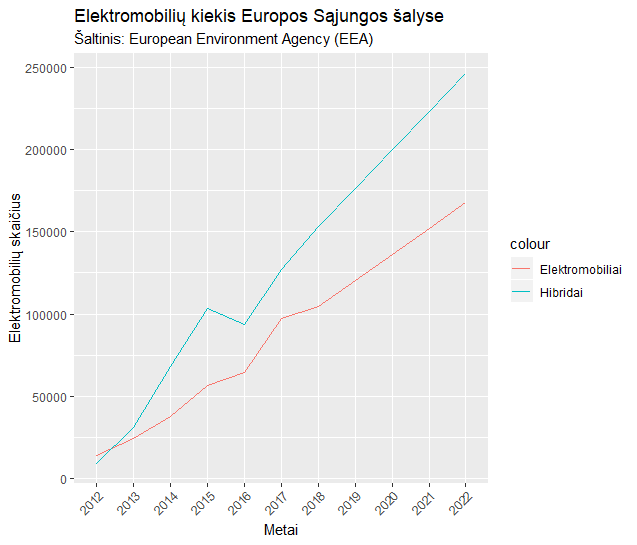
\includegraphics[scale=1]{elektromobiliai}
\end{figure}

Grafike galime matyti, jog paklausa didės tiek hibridų, tiek elektromobilių, pagal tai galima spręsti, kad elektra varomi automobiliai užims vis didesnę transporto rinkos dalį Europos Sąjungos šalyse. Nors spėjama, kad ištobulinus elektromobilių technologiją ir sukūrus geresnę bateriją tik elektra varomų automobilių kiekis bus didesnis už kitų tipų, dabar galima matyti hibridinių automobilių paklausos greitą augimą. Hibridiniai automobilių kiekis sumažėjo 2015m, tačiau nuo 2016m. pradėjo sparčiai didėti.  Remiantis šia prognoze 2022m. elektromobilių bus beveik 170 000, o hibridų 250 000. Ateityje elektriniu varikliu varomų transporto priemonių pardavimai turėtų dar labiau didėti.

\newpage
\section{Pokytis elektros rinkoje}

Pirmoje rašto darbo dalyje aptarta elektra varomų transporto priemonių paklausa bei prognozės. Pateikta prognozė, jog tokio tipo automobilių kiekis augs ir galiausiai jie užims didžiausią dalį parduodamų transporto priemonių rinkos. Atsižvelgus į šiuos spėjimus, elektromobilių kiekiui didėjant susiduriama su naujomis problemomis. 
Visų pirma, dabartiniai elektros energijos tinklai vietovėse, kuriose eismo srautai yra dideli, tačiau neturi didelės elektros energijos paklausos, turės sunkumų susidorodami su paklausos padidėjimu. Todėl vyriausybei gali tekti išplėsti perdavimo linijas arba pertvarkyti dabartinį elektros energijos gamybos portfelį, kad būtų užtikrintas elektros tinklo stabilumas.\parencite{moon2018forecasting}
Dar viena problema, elektrinėms reikės tiekti daugiau energijos visoje šalyje, net nuošaliausiose vietovėse bus reikalingos įkrovimo stotelės.

\subsection{Kaip pasikeis elektros paklausa transporto sektoriuje?}
Kaip keisis elektros energijos paklausa transporto sektoriuje lemia įvairios priežastys. Viena iš jų yra elektrinių variklių diegimas ne tik lengvuosiuse automobilius, bet ir autobusuose, traukiniuose. Elektromobilių kainos taip pat daro įtaką elektros paklausai, nes elektromobilių kainoms esant lygioms arba nelabai didesnėms kaip tokio pat galingumo automobilio, varomo vidaus degimo varikliu, pirkėjai pagal Hyung Bin Moon atliktą analizę mieliau rinktųsi elektra varomus automobilius. Tai parodo, jog pasikeitus kainai elektromobilių kelyje daugėtų, todėl reikėtų vis daugiau įkrovimo stotelių. 
Be to, svarbu kaip keisis keleivių transporto sektorius.
Ateities keleivių transporto sektoriaus plėtra aptariama šešiais scenarijais; tai yra bazinis scenarijus, besivystančio viešojo transporto scenarijus, kuriamų naujos ir švarios energijos transporto priemonių scenarijus, lengvinantis kelių perkrovą scenarijus, transporto pasidalijimo scenarijaus ir optimalus scenarijus.\parencite{fan2017energy}
Visi šie scenarijai skirti tam, kad būtų sukurtas naujas ekologiškesnis transporto sektorius. Priklausomai nuo scenarijaus skiriasi ir nuspėjamas elektros poreikis transporto sektoriuje. Pavyzdžiui, kuriamų naujos ir švarios energijos transporto priemonių scenarijaus atveju elektros paklausa ženkliai padidės, kadangi elektra varomų autobusų paklausa turėtų padidėti iki 30proc. ir kristi dyzelinių autobusų paklausa. Renkantis scenarijus, kuriuose šalies valdžia įsipareigoja priimti įstatymus dėl nulinės taršos zonų, taip skatindamos rinktis ekologiškesnes transporto priemones, elektros paklausos kiekis didėja greičiau. Galima teigti, jog elektros paklausa tikrai didės, tačiau kaip sparčiai keisis priklauso nuo įvairių aplinkybių: elektromobilių paklausos, valdžios priimamų įstatymų bei bendros šalių politikos. Preliminarus elektros paklausos keitimasis, neatsižvelgiant į valstybės politiką, atvaizduotas grafike. 

\newpage
\begin{figure}[h]
\centering
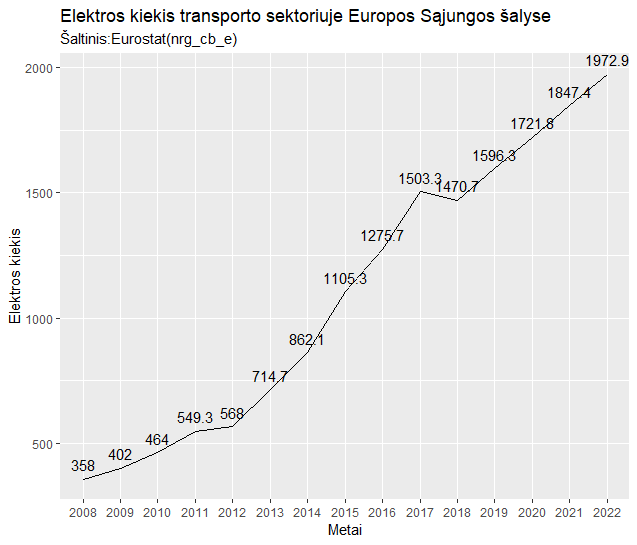
\includegraphics[scale=1]{elektra.png}
\end{figure}

Grafike galima pastebėti, kad elektros paklausa Europos Sąjungoje transporto sektoriuje didėja nuo 2008m., spartesnis augimas pastebimas nuo 2012m. Nuo 2017m. elektros paklausos kiekis pradėjo mažėti, tačiau nuo 2018m. vėl didėjo. Pagal šiuos skaičiavimus 2022m. elektros paklausa turėtų pasiekti beveik 2000 gigavatų per valandą. Galima spėti, kad elektros paklausa augs vis sparčiau ypač, jeigu bus kuriamos nulinės taršos zonos ir kuriama gera infrastruktūra elektromobiliams šalyse. Elektros energijos kiekio didėjimas transporto sektoriuje yra akivaizdus bei iškelia naujus klausimus dėl kainų bei ekologijos.


\subsection{Elektros paklausos pasikeitimo pasekmės}
Pagal padarytus skaičiavimus matoma, jog elektros paklausa didės. Tai padeda efektyviau išnaudoti elektros perdavimo infrastruktūrą, kas gali mažinti elektros kainą. Tačiau Viktorija Bobinaitė ir Aldona Juozapavičienė atliko elektros energijos rinkos kainos savybių tyrimą ir padarė išvadas. Teoriniu lygmeniu atlikus elektros energijos kainos
savybių formavimosi priežasčių analizę, galima teigti, kad
elektros energijos kainos savybės pasireiškimas (nepasireiškimas) priklauso nuo to, kaip kainą paveikia veiksniai,
darantys įtaką elektros energijos pasiūlai ir paklausai. Taigi
visus veiksnius, veikiančius elektros energijos kainos savybių pasireiškimą, galima sugrupuoti pagal veiksnių sąryšį su
rinkos paklausa, pasiūla ir rinkos struktūra. Elektros energijos kaip prekės savybės taip pat veikia elektros energijos
kainą ir jos savybių formavimąsi.
Žiemos laikotarpiu, kai prekybą rinkoje vykdo šiluminės
elektrinės, kainos kaitumas mažėja, tačiau vidutinis kainų
lygis kyla. Pavasarį, esant galimybei importuoti elektros
energiją pigiau, kainos kaitumas didėja, o vidutinis kainų
lygis mažėja.\parencite{juozapavivciene2012analysis}
Galima teigti, kad nuspėti, kaip elektromobilių paklausos kiekio didėjimas paveiks elektros kainą, yra labai sudėtinga ir priklauso ne tik nuo elektromobilių skaičiaus didėjimo, bet ir nuo kitų veiksnių. 
Jeigu elektros energijos kaina didės, vartotojai gali norėti sumažinti savo transportui skirtas išlaidas. Tai gali juos paskatinti įsigyti saulės kolektorius, kurie ne tik dar labiau mažins šio vairuotojo taršą, bet ir leis vairuotojui naudotis nemokama elektros energija. Saulės kolektorių pagamintą elektrą galima naudoti ne tik pakrauti elektromobilį, bet ir namų buityje. Padidėjus elektros gamybai namuose šiuo būdu, vartotojai taps ekologiškesni ir tikriausiai toks elektros gamybos būdas juos paskatins rinktis tik elektromobilius ypač saulėtose šalyse.

\newpage
\sectionnonum{Išvados}
Šio straipsnio tikslas buvo apžvelgti elektra varomų elektromobilių ir elektros transporto sektoriuje paklausas Europos Sąjungoje ir atlikti preliminarias prognozes, kaip keisis paklausos kiekiai. Pagal atliktas prognozes paaiškėjo, kad tiek hibridų, tiek visiškai elektra varomų transporto priemonių kiekis Europos Sąjungoje didės. Šis pokytis lems pasikeitimus ir elektros rinkoje. Elektros energijos paklausa didės transporto sektoriuje, ypač spartus augimas turėtų būti, jeigu valstybės priims nulinę taršą skatinančius įstatymus. Galima daryti tokias išvadas, jog elektromobilių skaičiaus didėjimas, didina elektros paklausos kiekį transporto sektoriuje, kuris gali keisti elektros kainą, kuri skatintų vartotojus gaminti elektros energiją namuose. Taip pat svarbu paminėti, kad elektromobilių paklausos didėjimas yra pagrindinė elektros paklausos didėjimo priežastis.

\newpage
\printbibliography[heading=bibintoc, title=Literatūros sąrašas]

\end{document}
